\chapter{Literature Review}

Following the initial work done by Axelrod, there are many other papers that
have tried to tackle the PD and make their conclusions on cooperation in both a
theoretical and real life setting. In this chapter a review of some of this work
done in the IPD competitions, in spatial and evolutionary game theory will be
carried out.
% I find it easier to avoid we/I etc.

\section{Tournaments}

In order to get an understanding of how to play the game of the Prisoner's
% I think that's probably an oversimplification of his motivation.
Dilemma better, Robert Axelrod held a tournament in 1980 ref. He invited a
number of well-known game theorists to submit strategies for a computer
tournament.  Each strategy has to specify whether to cooperate or defect based
on the history of previous moves made by both players.  Strategies played again
each other as well as a further Random strategy, that would randomly choose
between C and D and with its own twin. The tournament was a round robin and all
entries new the exact length (200 moves) of each game.  Fourteen strategies were
submitted and by the end Tit for Tat was announced the winner. Surprisingly in
% Same comment about TfT: the reader does not know what this is
the second tournament held where 64 strategies competed and all submitters had
full knowledge of what have happened in the first tournament, Tit for Tat
managed to get first place again.\parencite{Axelrod1980a}

Tit for Tat is a deterministic strategy that will always cooperate in the first
% Cool so here is your explanation of it but the reader will be confused with no
% pointers that it is coming.
round and afterwards it copies the opponents last move. Surprisingly in the
second tournament held by Axelrod \parencite{Axelrod1980a} where 64 strategies
competed and all they writes had full knowledge of what have happened in the
first tournament, Tit for Tat managed to get first place again.
% This is a repetition of the previous paragraph.
As explained in \parencite{Axelrod1980b}, Tit for Tat, a simple strategy was
able to beat sophisticated and more complex strategies thanks to three
specific characteristics of the strategy:

\begin{itemize}
  \item Niceness:  A strategy is categorized as nice if it was not the
                    first to defect, or at least, it will not do this until
                    the last few moves.
  \item Forgiveness: The propensity to cooperate in the moves after the
                     opponent defected.
  \item Clarity: After opponents identified that they were playing Tit for Tat
                 choose to cooperate for the rest of the game.
\end{itemize}

The first tournaments were an innovation in combining computer modeling and Game
Theory and in providing insights in the behavior emerging from simple dynamics.
Moreover, Axelrod was the first to speak about niceness, forgiveness and gave an
illustration that cooperation can be a victorious and advantageous strategy.

There have been other tournaments, based off of Axelrod’s, exploring different
environments and submitting new strategies. In 1991 Bendor, Kramer and Stout
% Reference properly (I know your references are a mess just trying to make sure
% they're not missed).
introduced noise to the IPD. Where noisy randomly flip the choice made by a
strategy.  Kerts 2011 conducted a tournament where the payoff matrix was altered
though satisfying the conditions (1.1), (1.2) . In 1992, Nowak and May
reproduced the first tournament with a spatial topology.
% You are repeating yourself right? You mentioned this in the first chapter.
Furthermore, some review tournaments are listed below:

% Do you think is a good idea to add a table with tournaments ?
% Yup.

\begin{table}[h]
\centering
\caption{An example table using the `booktabs' package}
\label{fig:exampletable}
\begin{tabular}{cccccccccc}
\toprule
& \multicolumn{3}{c}{\textbf{ABC}} & \multicolumn{3}{c}{\textbf{ABC}} & \multicolumn{3}{c}{\textbf{ABC}} \\
\cmidrule(lr){2-4}\cmidrule(lr){5-7}\cmidrule(lr){8-10}
\textbf{Example}      & \textbf{A}       & \textbf{B}       & \textbf{C}      & \textbf{A}           & \textbf{B}           & \textbf{C}          & \textbf{A}           & \textbf{B}           & \textbf{C}          \\
\cmidrule(lr){1-1}\cmidrule(lr){2-4}\cmidrule(lr){5-7}\cmidrule(lr){8-10}
0         & 1234      & 1234     & 1234     & 1234          & 1234         & 1234         & 1234        & 1234         & 1234         \\
1         & 1234      & 1234     & 1234     & 1234          & 1234         & 1234         & 1234        & 1234         & 1234         \\
2         & 1234      & 1234     & 1234     & 1234          & 1234         & 1234         & 1234        & 1234         & 1234        \\
3         & 1234      & 1234     & 1234     & 1234          & 1234         & 1234         & 1234        & 1234         & 1234         \\ \bottomrule
\end{tabular}
\end{table}

% Add a sentence or two saying what you've said in this section and introducing
% the next one (think of your reader as someone you're helping across the
% street: help them on every step).

\section{Spatial Structure Tournaments}

Further research was spawn in 1992 as to how the Prisoner's Dilemma could shade
some insight into physics and biology. Where they believed exist potential
dynamics of spatially extended systems. Their tournament was a simple and purely
% 'Their': who is they? You're missing the reference somewhere here.
deterministic spatial version of the PD in a two dimensional lattice. With
players having no memory of the previous rounds and no strategical elaboration.
Thus, the players could either always cooperate or defect. The local winner of
each generation would win a territory. His neighbors would follow his strategy.
% What does 'win a territory mean': be precise.  Don't use he/him (masculin).
% Either be diverse so use he/her she/him or be neutral (be neutral). This is
% often tricky for writer whose first language has masculin and feminin nouns.
% In english nouns are neutral.
This allowed them to generate spatial chaotic patterns: these patterns depended
on the Temptation payoff (\(T\)). \cite{Nowak and May} concluded that co-operational
behavior is possible in the PD by using a spatial topology.
% Why how? What does this last sentence have to do with chaotic patterns?

Similarly, in \parencite{Lindgren1994} players were allowed to have
% Not similarly right? This was the main difference.
memory and therefore added complex strategies to the tournament such as Tit for
Tat and  Anti Tit for Tat. This was followed  by the work of
\parencite{Brauchli1999} which introduced even more
complex strategies.
% What were the conclusions of these pieces of work?

Spatial topology has been defined by most scholars as a square lattice where
the nodes - players only interact with their neighborhoods. Including connections
between four or eight nearest neighbor sites, Neuman's or Moore's, according to
Figure~\ref{fig:neighborhood}. A square lattice is a graph and one could argue
that a round robin tournament itself is the complete graph on all players
(\cite{some general book about graph theory}). But in the above papers
no authors defined the topology as a graph, apart from \parencite{Meng2015}.

In \parencite{Meng2015}, an interesting approach was used. They presented a new
spatial prisoner's dilemma game model in which the neighborhood size was
increased onto two interdependent lattices. They implement the utility by
integrating the payoff correlations between two lattices. A player would mimic a
random player in his next move, base on a function that consider the utility of
the player. It was characterized as a most realistic scenario.

Real life interactions are more likely to be like any given graph depending on
the industry than a complete graph. Fatha et all, have considered a numerous of graphs,
% Reference properly
such as :

\begin{itemize}
  \item Lattice, the interaction network is defined by the sites of a lattice.
   the distance between a pair does not exceed a given value.
   The most frequently used structure is the square lattice with von Neumann
   neighborhood and Moore neighborhood.
  \item Small word, a graph that is created from a square lattice by randomly
   rewiring a fraction of connections in a way that conserve the degree for
   each site.
  \item Scale-free graphs, a network that has a power-law degree distribution, regardless of
   any other structure.
  \item Evolving networks, networks that change as a function of time (this will
      not be considered in this dissertation).
\end{itemize}

The major theme of their review was how the graph structure of interactions could
modify long term behavioral patterns emerging in evolutionary games.
These graphs compose only a small fraction of graphs that exist. In this
dissertation we will consider a list of graphs.
 %add list when i actually know

\section{Axelrod Python Library}

The Axelrod library (.ref) is an open source Python package that allows for
reproducible game theoretic research into the Iterated Prisoner's Dilemma[url].
For many of the tournaments aforementioned the original source code is almost never
available and in no cases is the available code well-documented, easily modified
or released with significant test suites. Due to that reproducing the results
has not been an easy task.

However, Axelrod library manages to provide such a resource, with facilities for
the design of new strategies and interactions between them, as well as
conducting tournaments and ecological simulations for populations of strategies.

Strategies are implemented as classes which have a single method, strategy().
It only takes one argument, which is the opponent's previous moves and returns
an action. These actions can be either to cooperate C or to defect D. At thins
moment the Axelrod library consists of 131 strategies.Can be found in the Appendix.

Additionally, tournament are classes responsible for running a repetition of a
round robins. It achieves that by calling a match generator class which
returns all the single match parameters, such as turns, the game and the noise.
Axelrod has the capability to write out the results into a csv file and also out
put plots with the ranks of the strategies.

Furthermore, a basic tournament of 200 turns, 100 repetitions and the 131
strategies that exist in the library is being produced continuously. The current
winner is called PSO gambler and it is a look up strategy. It uses a lookup
table with probability numbers generated using a Particle Swarm Optimisation
(PSO) algorithm.  Here are illustrated the results of the last tournament :
% If you go to the documentation list for the strategies you can find a url
% describing how this was done you should reference that.

\begin{figure}[h]
\centering
    \begin{subfigure}[t]{0.55\textwidth}
    \centering
        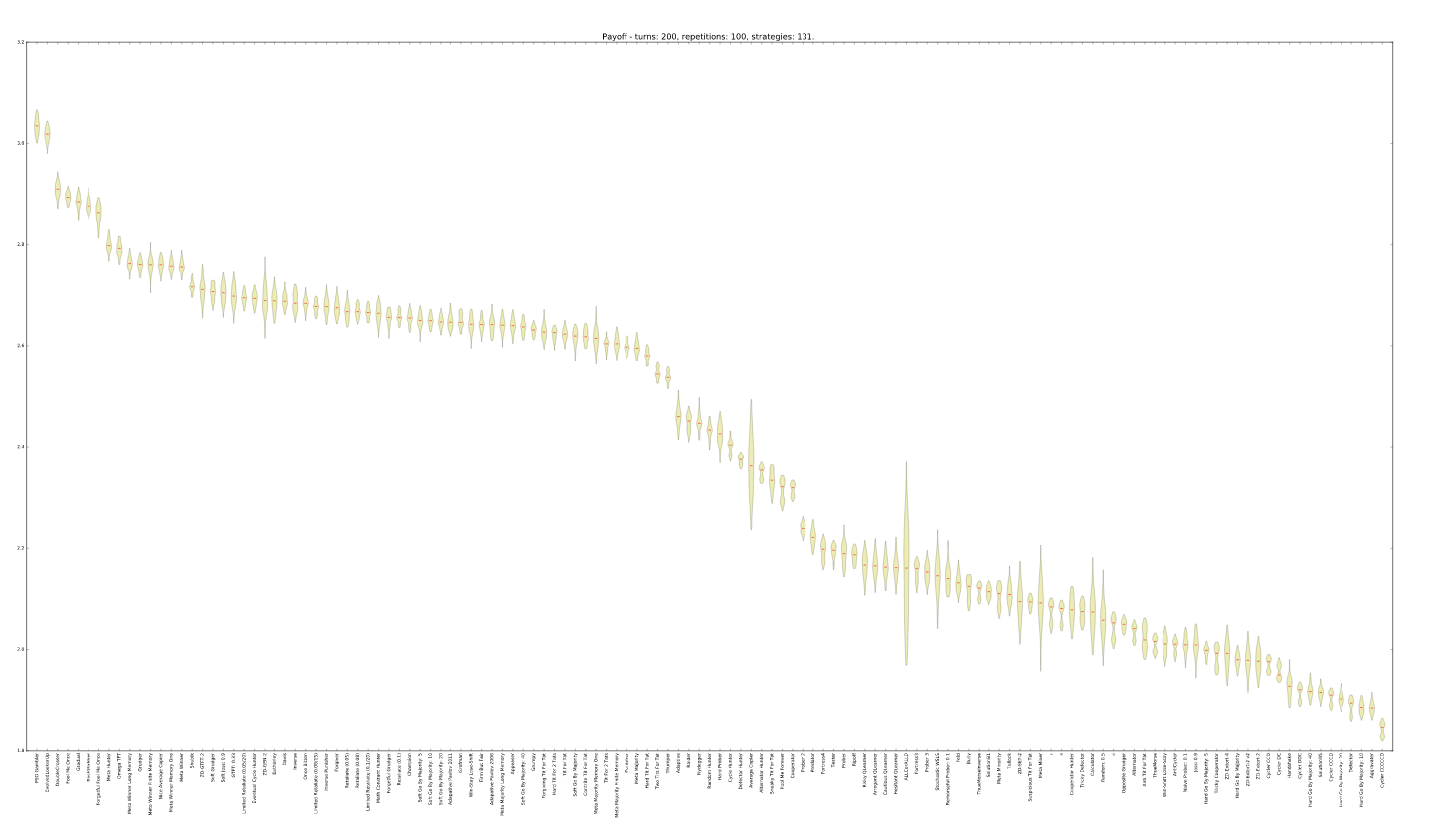
\includegraphics[width=\linewidth]{axl.png}
    \caption{Ranked violin plot}
    \end{subfigure}
\hfill
    \begin{subfigure}[t]{0.50\textwidth}\centering
    \centering
        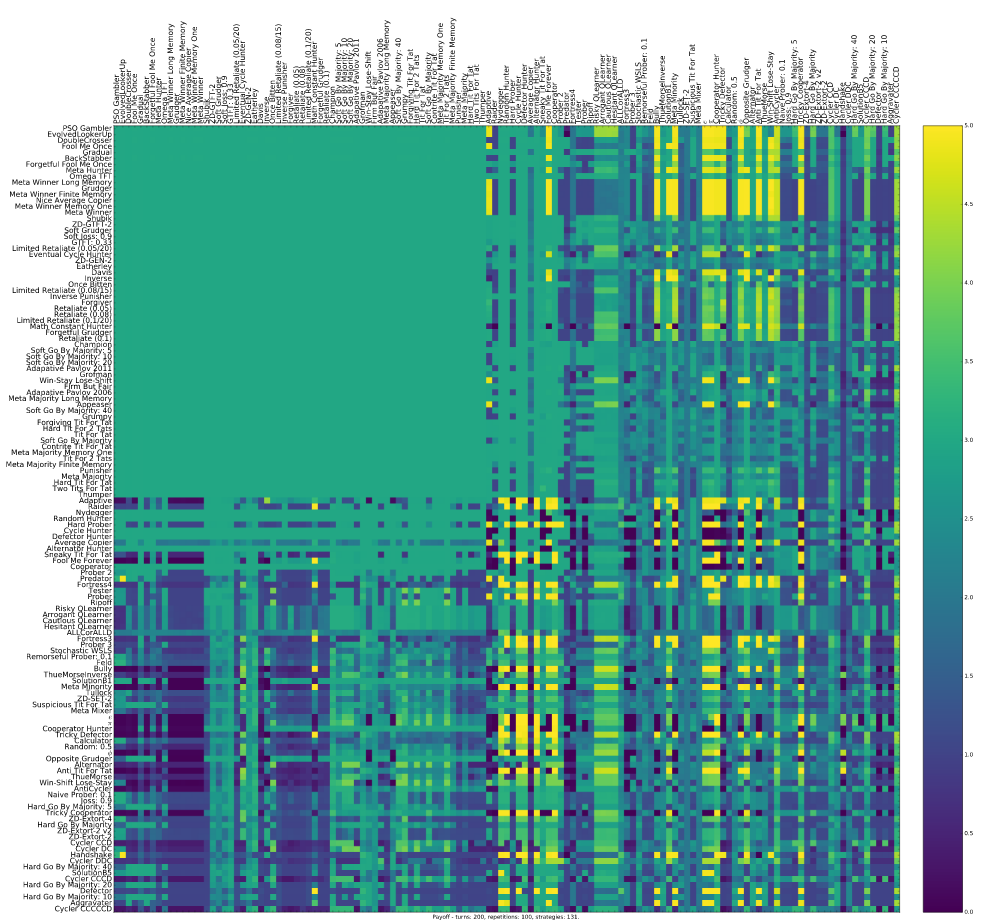
\includegraphics[width=\linewidth]{axl1.png}
    \caption{Payoffs}
    \end{subfigure}
~
\caption{Result Plots. (a) Ranked violin plot, the mean utility of each player.
(b) Payoffs, the pair wise utilities of each player.}
\label{fig:axelrodplots}
\end{figure}

Because is an open source library it makes it easy to contribute to it and
make modifications needed for this dissertation.


% This section on the library can/will be rewritten. See comment in chapter 1
% about citation.
